%-------------------------------------------------------------
%  INTRODUCTION
%-------------------------------------------------------------

Maude~\cite{CDELMMQ:2002,CDELMMT:2007-book} is an executable formal specification language based on rewriting logic, which counts with a rich set of validation and verification tools~\cite{CDELMMT:2007-book,CDHLMO:2007}, increasingly used as support to the development of UML, MDA, and OCL tools (see, e.g., \cite{Boronat-Meseguer:08,RRDV:07-jot,Clavel-Egea:06}). Furthermore, Maude has demonstrated to be a good environment for rapid prototyping, and also for application development (see surveys~\cite{CDELMMT:2007-book,Meseguer:2012}). 

Maude may be seen as a general framework where to develop model transformations. Thus, Meseguer and Boronat use it to implement their model transformation framework MOMENT2; Dur\'an, Vallecillo and others have used it to develop e-Motions~\cite{RiveraDV10}, a tool that supports the definition and simulation of real-time Domain-Specific Modeling Languages (DSMLs); and similar approaches have later been used to give semantics to ATL~\cite{TroyaV10} and other transformation languages. 

The e-Motions tool is a DSML and graphical framework developed for Eclipse that supports the specification, simulation, and formal analysis of real-time systems. It provides a way to graphically specify the dynamic behavior of DSMLs using their concrete syntax, making this task quite intuitive. Furthermore, e-Motions behavioral specifications are models too, so that they can be fully integrated in MDE processes.

In e-Motions, MOF metamodels are formalized in rewriting logic, providing a representation of the structural aspects of any modeling language with a MOF metamodel. Then, given a description of the behavior of such modeling language as in-place transformation rules, e-Motions may be used to define both the syntax and the operational semantics of DSMLs. Artifacts developed in e-Motions are automatically translated into Maude.

As we will see in the following sections, e-Motions provides a very rich set of features, that enables the formal and precise definition of real-time DSMLs as models in a graphical and intuitive way. It makes use of an extension of in-place model transformation with a model of timed behavior and a mechanism to state action properties. The extension is defined in such a way that it avoids artificially modifying the DSML's metamodel to include time and action properties. Moreover, it supports attribute computations and ordered collections, which are specified by means of OCL
expressions, thanks to mOdCL~\cite{Roldan-Duran:2008-tr}. All these features makes the language very expressive, but directly impact on performance. To gain an idea of this impact, we provide below solutions to the proposed problems both in e-Motions and directly in Maude and compare them. 

The e-Motions system documentation and several examples are available at \url{http://atenea.lcc.uma.es/e-Motions}. The Maude web site is at \url{http://maude.cs.uiuc.edu}.

\subsection{e-Motions}\label{sub:emotions}

The definition of a Domain-Specific Language (DSL) typically comprises three tasks: (i) the definition of its abstract syntax, (ii) the definition of its concrete syntax and (iii) the specification of its behavior.

In e-Motions the abstract syntax is defined by means of an Ecore metamodel, in which all the language concepts and the relations between them are specified. The concrete syntax is provided by defining the so-called Graphical Concrete Syntax (GCS). A GCS is a model (conforms the GCS metamodel) where an image is attached to each concept defined in the abstract syntax.

In e-Motions the behavior of a DSL is specified using visual graph-transformation rules. An e-Motions rule consists of a\delete{---possibly conditional---} Left-Hand Side (LHS), a Right-Hand Side (RHS) and zero or more Negative Application Conditions (NACs). The LHS defines a (sub)-graph matching, optionally conditional. The RHS specifies a (sub)-graph replacement, which if the rule is applied, every object in the LHS that is not in the RHS is deleted, new objects in the RHS that are not in the LHS are created, and those objects whose attributes (or links) are changed are updated. NACs specify conditions or (sub)-graphs such that if there is a matching, the rule cannot be fired.

Figure~\ref{fig:assemble} shows an example of an e-Motions rule. The objects in both the RHS and LHS are represented by their associated images, as defined in the GCS model. Rule \code{Assemble}'s LHS defines the precondition of the rule. It models an assemble machine who needs both a head and a handle in its connected conveyor. If \code{NAC1}, stating that the current matched \code{Assemble} object is not involved in other \code{Assemble} action, is not satisfied, the rule can be applied. The rule is applied as follows. All objects in its LHS which do not appear in its RHS are deleted, i.e., objects \code{he} and \code{ha}. Those objects in its RHS which do not appear in its LHS are created, properly setting their attributes, i.e., the \code{ham} object with its three attributes. The rest of the objects remain changeless. Moreover, as e-Motions is a framework where to define real-time systems, each rule is applied in a established time, i.e. \code{[prodTime,prodTime]} in the \code{Assemble} rule. A rule with execution time \code{[0,0]} is considered instantaneous. A rule may contain zero or more local or auxiliary variables. All attribute or variable assignments and conditions are expressed using Object-Constraint Language (OCL)~\cite{ocl}.

The abstract and concrete syntax, and the behavior of a DSL are models, and the e-Motions tool has been developed following MDE principles. The Maude code corresponding to a system defined in e-Motions is generated by an ATL/TCS transformation~\cite{ATL}.

\begin{figure}[htp]
  \centering
  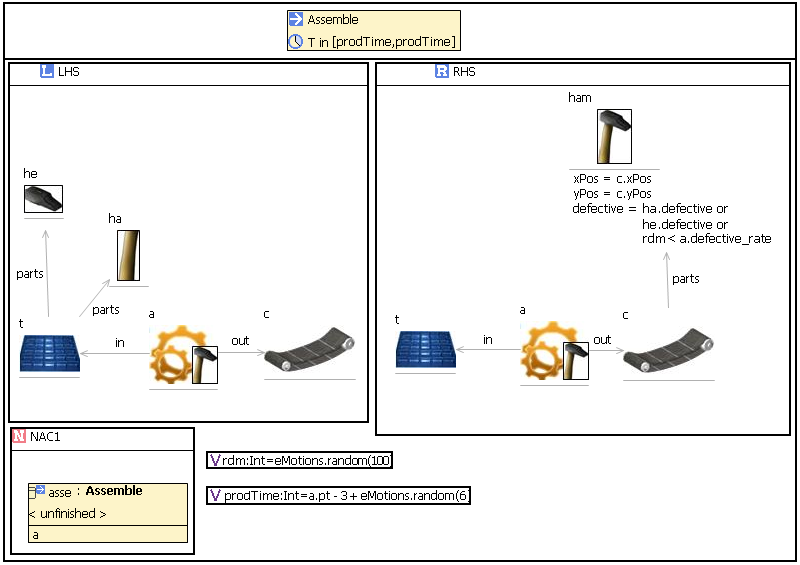
\includegraphics[width=\textwidth]{imgs/assemble}
  \caption{e-Motions \code{Assemble} rule.}\label{fig:assemble}
\end{figure}

\subsection{Rewriting Logic and Maude}

Rewriting logic (RL)~\cite{Meseguer:92-tcs} is a logic of change
that can naturally deal with state and with highly nondeterministic
concurrent computations.
In RL,  the state space of a distributed system is specified as an
algebraic data type in terms of an equational specification
$(\Sigma,E)$, where $\Sigma$ is a signature of sorts (types) and
operations, and $E$ is a set of equational axioms. The dynamics of a
system in RL is then specified by rewrite \emph{rules} of the form
$t \rightarrow t'$, where $t$ and $t'$ are $\Sigma$-terms.
This rewriting happens modulo the equations $E$, describing in fact
local transitions $[t]_E\rightarrow[t']_E$.
These rules describe the local, concurrent transitions possible in the
system, i.e. when a part of the system state fits the pattern $t$
(modulo the equations $E$)
then it can change to a new local state fitting pattern $t'$.
Notice the potential of this type of rewriting, and the very high-level of
abstraction at which systems may be specified, to perform, e.g.,
rewriting modulo associativity or associativity-commutativity.

Maude~\cite{CDELMMQ:2002,CDELMMT:2007-book} is a
wide spectrum programming language directly based on RL.
Thus, Maude integrates an
equational style of functional programming with RL computation.
Maude also supports the modeling of object-based systems by providing
sorts representing the essential concepts of object
(\texttt{Object}), message (\texttt{Msg}), and configuration
(\texttt{Configuration}). A configuration is a multiset of objects
and messages (with the empty-syntax, associative-commutative, union
operator \verb~__~) that represents a possible system
state.

Although the user is free to define any syntax for objects
and messages, several additional sorts and operators are introduced
as a common notation. Maude provides sorts \texttt{Oid} for object
identifiers, \texttt{Cid} for class identifiers, \texttt{Attribute}
for attributes of objects, and \texttt{AttributeSet} for multisets
of attributes (with \verb~_,_~ as union operator).
Given a class $C$ with attributes $a_i$ of types $S_i$, the objects
of this class are then record-like structures of the form

$$\texttt{<} \; O \; \texttt{:} \; C \; \texttt{|} \; a_1 \texttt{:}
v_1 \texttt{,} \; ... \texttt{,} \; a_n \texttt{:} v_n \;
\texttt{>}$$

\noindent where $O$ is the identifier of the object, and $v_i$
are the current values of its attributes (with appropriate types).
See \cite{CDELMMT:2007-book} for additional details on how
object-oriented systems are represented in Maude, including
explanations on how to represent inheritance, syntax for
object-oriented modules, different forms of object communication,
etc.

The following Maude definitions specify a class
\texttt{Account} of bank accounts, with messages \verb"withdraw" and
\verb"transfer" to operate with such bank accounts. The
\verb"Account" class is defined with a single attribute
\verb"balance", of sort \verb"Int", representing the balance of an
account. The \verb"withdraw" message has two parameters, namely the
addressee of the message and the amount of money to withdraw from
the account. The \verb"transfer" message will make the amount of
money specified as its third argument to be transferred from the
account given as first argument to the one given as second argument.

{\small
\begin{verbatim}
  sort Account .
  subsort Account < Cid .
  op Account : -> Account .
  op balance :_ : Int -> Attribute .
  op withdraw : Oid Int -> Msg .
  op transfer : Oid Oid Int -> Msg .
\end{verbatim}
}

\noindent Rules \verb"debit" and  \verb"transfer" below represent local
transitions of the system that specify the behavior of bank accounts
upon the reception of such messages. E.g., if an \verb"Account"
object receives a \verb"withdraw" message and the amount of money to
withdraw is smaller or equal than the balance of the account
receiving the message, then the message is `consumed' and the
balance of the account is decremented is such an amount. Notice the
synchronization of \verb"Account" objects in the \verb"transfer"
rule.

{\small
\begin{verbatim}
  vars A B : Oid .
  vars BalA BalB M : Int .

  crl [debit] :
    < A : Account | balance : BalA >
    withdraw(A, M)
    => < A : Account | balance : BalA - M >
    if BalA >= M .
  crl [tranfer] :
    < A : Account | balance : BalA >
    < B : Account | balance : BalB >
    withdraw(A, M)
    => < A : Account | balance : BalA - M >
       < B : Account | balance : BalB + M >
    if BalA >= M .
\end{verbatim}
}

\noindent Notice that, since the \verb"__" operator is declared associative,
commutative, and with identity element, we do not need to worry about the order
in which objects and messages appear in the rules.
And since rules describe local transitions, we do not need to worry
about the rest of the objects and messages in the configuration either.

Well-formedness of objects may be automatically checked by Maude's typing system.
For example, we can add declarations constraining \verb"Account" objects:

{\small
\begin{verbatim}
  sort AccountObject .
  subsort AccountObject < Object .

  var O : Oid .
  var Bal : Int .

  mb < O : Account | balance : Bal > : AccountObject .
\end{verbatim}
}

\noindent Notice that with these declarations, an object
  \verb"< O : Account | >"
is a valid term of sort \verb"Object", but since the membership cannot be applied on it,
it is not of type \verb"AccountObject".

